% Lines that start with a % are comments and are not included when the LaTeX file is converted to a pdf

% Set up the document class - this can be changed if a different format is required 
\documentclass[12pt,a4paper]{article}

% Include packages that contain additional features, for example including special mathematical characters and images in your document
\usepackage{amssymb,amsmath,graphicx}


\usepackage{geometry}
 \geometry{
 a4paper,
 total={170mm,257mm},
 left=20mm,
 top=20mm,
 }



% The beginning of the document...
\begin{document}

% Please change the following accordingly...
\centerline{\large Exercise sheet 5}\vspace{0.5em}
\centerline{\large by Maximilian Richter and Christian Heppe}\vspace{1em}

% Split the different exercises into different sections...
\section*{Pertubated quantum mechanical oscillator}
Consider a dimensionless Hamiltonian 
\begin{equation}
h=\frac{H}{\hbar\omega}=\left(\frac{1}{2}\Pi^2+\frac{1}{2}Q^2+\lambda Q^4\right)
\end{equation}
\begin{equation}
(h)_{nm}=(h_0)_{nm}+\lambda(Q^4)_{nm}
\end{equation}
where 
\begin{equation}
(h_0)_{nm}=\left(n+\frac{1}{2}\right)\delta_{nm}
\end{equation}
is the unperturbated Hamiltonian
% To include a plot it must be in the same directory as the .tex file.
\subsection*{a) Determining the matrix form of $Q^4$}
Using
\begin{equation}
Q_{nm}=\frac{1}{\sqrt{2}}\left(\sqrt{n+1}\delta_{n,m-1}+\sqrt{n}\delta_{n,m+1}\right)
\end{equation}
and the properties of the creation and annihilation operator $a$ and $a^{\dagger}$ we can obtain $Q^4$ with the following approach:
\begin{align*}
(a+a^{\dagger})|n\rangle=&\sqrt{n+1}|n+1\rangle+\sqrt{n}|n-1\rangle\\
(a+a^{\dagger})^2|n\rangle=&\sqrt{(n+1)(n+2)}|n+2\rangle+(2n+1)|n\rangle+\sqrt{n(n-1)}|n-2\rangle\\
(a+a^{\dagger})^3|n\rangle=&\sqrt{(n+1)(n+2)(n+3)}|n+3\rangle+(3n+3)\sqrt{n+1}|n+1\rangle\\
&+3n\sqrt{n}|n-1\rangle+\sqrt{n(n-1)(n-2)}|n-3\rangle\\
(a+a^{\dagger})^4|n\rangle=&\sqrt{(n+1)(n+2)(n+3)(n+4)}|n+4\rangle+(4n+6)\sqrt{(n+1)(n+2)}|n+2\rangle\\
&+(6n^2+6n+3)|n\rangle+(4n-2)\sqrt{n(n-1)}|n-2\rangle+\sqrt{n(n-1)(n-2)(n-3)}|n-4\rangle
\end{align*}
This way we can finally derive the matrix representation of this expression by multiplying with the dual vector
\begin{equation}
(Q^4)_{mn}=\langle m|(a+a^{\dagger})^4|n\rangle
\end{equation}
and using the relation
\begin{equation}
\langle m|n\rangle=\delta_{mn}
\end{equation}
we can find
\begin{align}
(Q^4)_{mn}=&\sqrt{(n+1)(n+2)(n+3)(n+4)}\delta_{m,n+4}\\
&+(4n+6)\sqrt{(n+1)(n+2)}\delta_{m,n+2}\\
&+(6n^2+6n+3)\delta_{m,n}\\
&+(4n-2)\sqrt{n(n-1)}\delta_{m,n-2}\\
&+\sqrt{n(n-1)(n-2)(n-3)}\delta_{m,n-4}
\end{align}
\subsection*{b) Eigenvalues of the pertubated oscillator}
In order to find the eigenvalues of the pertubated oscillator, we started by defining the matrix $Q^4$, adding it to the unpertubated Hamiltonian, finding the tridiagonal form and finally finding the eigenvalues of the pertubated Hamiltonian using the off-diagonal elements of the tridiagonal matrix. $\lambda$ has been set to $\lambda=0.1$\\
Eigenvalues for $n=15$:
\begin{align*}
n = 0 : E_n &= 0.669\\
n = 1 : E_n &= 2.217\\
n = 2 : E_n &= 4.104\\
n = 3 : E_n &= 6.218\\
n = 4 : E_n &= 8.521\\
n = 5 : E_n &= 11.302\\
n = 6 : E_n &= 14.582\\
n = 7 : E_n &= 21.075\\
n = 8 : E_n &= 27.266\\
n = 9 : E_n &= 42.837\\
\end{align*}
Eigenvalues for $n=20$:
\begin{align*}
n = 0 : E_n &= 0.669\\
n = 1 : E_n &= 2.217\\
n = 2 : E_n &= 4.103\\
n = 3 : E_n &= 6.216\\
n = 4 : E_n &= 8.514\\
n = 5 : E_n &= 10.966\\
n = 6 : E_n &= 13.644\\
n = 7 : E_n &= 16.654\\
n = 8 : E_n &= 21.458\\
n = 9 : E_n &= 26.497
\end{align*}
Eigenvalues for $n=30$:
\begin{align*}
n = 0 : E_n &= 0.669\\
n = 1 : E_n &= 2.217\\
n = 2 : E_n &= 4.103\\
n = 3 : E_n &= 6.216\\
n = 4 : E_n &= 8.511\\
n = 5 : E_n &= 10.963\\
n = 6 : E_n &= 13.554\\
n = 7 : E_n &= 16.268\\
n = 8 : E_n &= 19.095\\
n = 9 : E_n &= 22.065\\
\end{align*}
\subsection*{c) Analytical solution}
To derive the analytical solution we use pertubation theory
\begin{equation}
\langle n|(a+a^{\dagger})^4|n\rangle=6(n^2+n+1/2)
\end{equation}
therefore we get a correction of the eigenvalues of
\begin{equation}
E_n'=\lambda6(n^2+n+1/2)
\end{equation}
So finally we get
\begin{equation}
E_n=E_0+E_n'=\left(n+\frac{1}{2}\right)+\lambda6(n^2+n+1/2)
\end{equation}
This yields
\begin{align*}
n = 0: E_n &= 0.8\\
n = 1: E_n &= 3\\
n = 2: E_n &= 6.4\\
n = 3: E_n &= 11\\
n = 4: E_n &= 16.8\\
n = 5: E_n &= 23.8\\
n = 6: E_n &= 32\\
n = 7: E_n &= 41.4\\
n = 8: E_n &= 52.\\
n = 9: E_n &= 63.8\\
\end{align*}
\begin{center}
%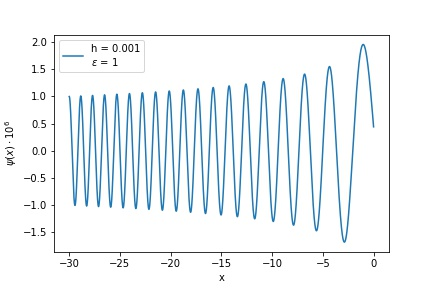
\includegraphics[width=8cm]{partb3.jpg}
\end{center}
\end{document}

